% Metódy inžinierskej práce

\documentclass[12pt,a4paper]{article}
\usepackage[numbers]{natbib}
\usepackage{url}
\usepackage{tocloft}
\usepackage{xcolor}
\usepackage{titlesec}
\usepackage[hidelinks]{hyperref}
\usepackage{pgfplots}
\usepackage{pgf-pie}
\usepackage[utf8]{inputenc}
\usepackage{lmodern} 
\usepackage{amsmath}
\usepackage{array}
\usepackage[utf8]{inputenc}
\usepackage{graphicx}
\usepackage{listings}
\usepackage{booktabs}
\usepackage{xcolor, colortbl}

\lstset{
    language=C,
    basicstyle=\ttfamily\small,
    keywordstyle=\color{blue}\bfseries,
    commentstyle=\color{gray},
    stringstyle=\color{red},
    numbers=left,
    numberstyle=\tiny\color{gray},
    stepnumber=1,
    numbersep=10pt,
    showspaces=false,
    showstringspaces=false,
    frame=single,
    tabsize=4,
    breaklines=true,
    breakatwhitespace=true,
    escapeinside={(*@}{@*)}
}


\usetikzlibrary{arrows.meta, positioning, shapes.geometric}
\pgfplotsset{compat=1.18}

\renewcommand{\cftsecleader}{\cftdotfill{\cftdotsep}}
\renewcommand{\cftsubsecleader}{\cftdotfill{\cftdotsep}}


\title{How Streaming Services Use AI and Algorithms to Personalize Your Music Experience}
\author{Mykyta Nosenko}
\begin{document}
\maketitle
\section*{Abstract}

Imagine you’re walking through a park, and everywhere you look, people are wearing headphones. Everyday, you can see hundreds or even thousands of individuals rapt in their own worlds of sound. What are they listening to? Some may be tuned into podcasts, audiobooks, or radio, but most are likely enjoying music. In today’s digital age, powerful streaming services like Spotify make accessing our favorite songs effortless. In this article, we will dive into how their recommendation systems work.

We’re about to explore the enormous world of algorithms and artificial intelligence that recommend songs specifically tailored to our tastes. At the heart of Spotify’s recommendation engine are algorithms like collaborative filtering and content-based filtering. For example, collaborative filtering uses matrix factorization to identify hidden user preferences based on listening habits, while content-based filtering employs techniques like TF-IDF to analyze song lyrics and extract significant themes. Additionally, Spotify leverages an AI system called Marlin, which combines these algorithms to enhance user experience and provide personalized music recommendations\citep{href}.

How do these systems understand our preferences? Who develops these complex technologies, and what exactly goes into building them? There are so many questions, and much remains unknown about how AI enhances our music experience, constantly adapting to our moods and listening habits. Let's take a closer look at how it all works.

\newpage
\tableofcontents
\newpage

\section{Recommendation Systems An Overview}



Greetings to everyone! I hope your mood is great and everything is going according to plan. Before we begin, try to clear your mind of distractions and fully immerse yourself in the topic. How do development teams within giants like Spotify, Yandex Music, Apple Music, and Deezer work — from solving complex tasks to team-building activities? Is machine learning involved? On what basis are recommendations made, and how do music services select the perfect playlists for us? So many questions, and there's so much to discover in this article. Let's dive in!

Modern music streaming services offer users not only access to extensive music catalogs but also ready-made playlists with personalized recommendations. Thanks to systems based on artificial intelligence and machine learning, the aforementioned platforms provide tracks that perfectly match each user's preferences. These systems play a crucial role in discovering new music. According to data from 2020, around 60\% (Refer to the diagram bellow) of users identified Spotify and YouTube as the main sources for finding new tracks and artists.Further details are provided in the diagram below \citep{href}\citep{Woman}.

Today, we will explore how recommendation systems work on the biggest music platforms — Yandex Music, Spotify, Apple Music, and Deezer. Each of them is unique and holds a leading position on its continent.

\begin{itemize}
 \item \textbf{Yandex Music} — the leading music service in Russia and the CIS countries, offers access to a vast collection of tracks and uses sophisticated algorithms to analyze your musical preferences and moods.

\item \textbf{Spotify}, a Swedish platform popular in Europe and America, is renowned for its smart playlists and recommendations based on your tastes, time of day, and even your mood.

\item \textbf{Apple Music} — a global giant, popular in the USA and many other countries, is tightly integrated into the Apple ecosystem. It uses your listening habits and interactions with music to create a personalized experience.

\item \textbf{Deezer}, a French leader, has gained popularity in Europe thanks to localized recommendations and unique algorithms that adapt music selections to each user as much as possible.
\end{itemize}

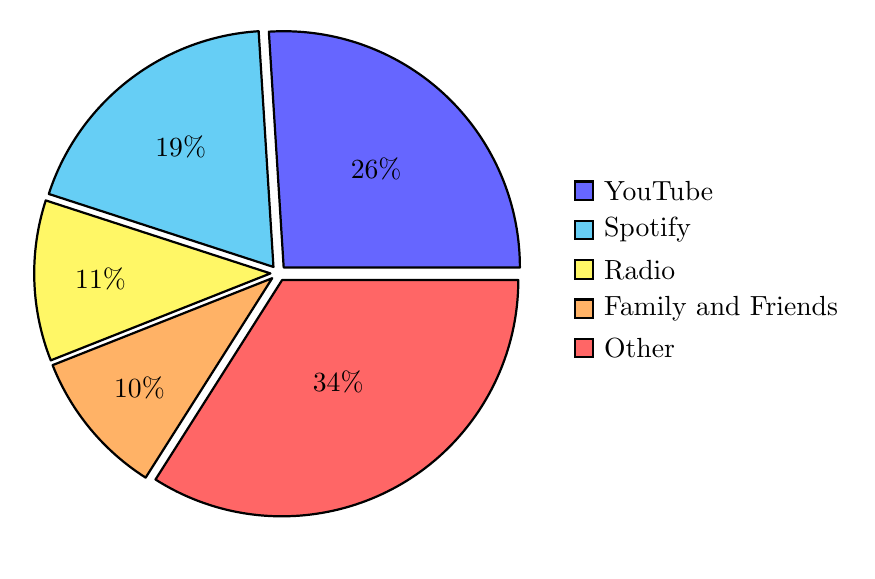
\begin{tikzpicture}
    \pie[
        text=legend, 
        radius=3, 
        explode=0.1 
    ]{
        26/YouTube,
        19/Spotify,
        11/Radio,
        10/Family and Friends,
        34/Other
    }
\end{tikzpicture}
\citep{Diagramm}

We have gathered information from podcasts and interviews with company executives and developers to better understand how these systems are built and what technologies power them. Ready to embark on a journey into the world of music technology? Let's go!

\section{Algorithms Behind the Recommendation Systems}
Spotify, with its vast library of over 82 million songs and 406 million subscribers, has transformed how listeners discover and engage with music. To tackle the overwhelming choices presented to users, Spotify employs sophisticated machine learning (ML) algorithms that not only recommend music but also enhance the overall listening experience. Here, we delve into the core algorithms used by Spotify, highlighting their functionalities and impacts\citep{key}.
\begin{itemize}
 \item \textbf{Collaborative Filtering (CF)}
Collaborative filtering is the cornerstone of Spotify's recommendation system. This technique relies on analyzing the collective behavior and preferences of users to predict what an individual might enjoy based on the actions of others with similar tastes. The sheer volume of playlists created by users—over 4 billion—provides a rich dataset for Spotify to extract insights.

User Clustering: Spotify identifies patterns in listening habits across various user clusters. For instance, if User A and User B frequently listen to similar artists, collaborative filtering allows Spotify to recommend new tracks to each user based on shared playlist behaviors.

Group Playlists: Spotify's acquisition of the music discovery company Tungio has enabled them to leverage both human intelligence and statistical methods to curate group playlists. These playlists are fine-tuned for performance, leading to increased user satisfaction.

Personal Playlist Personalization: By analyzing user engagement with personal playlists, Spotify can offer tailored recommendations. If User A adds a song by Bon Iver, the algorithm increases the likelihood of recommending Bon Iver tracks to User B, who has similar listening habits\citep{key}.

 \item \textbf{Natural Language Processing (NLP)}
Natural Language Processing allows Spotify to understand and categorize music based on textual data available on the internet. This includes song descriptions, reviews, and social media commentary. By employing NLP, Spotify can enhance its recommendation engine in the following ways:

Keyword Extraction: The algorithm scans and categorizes songs by extracting keywords and assigning them weights based on emotional context. This means that songs can be classified by the emotions they evoke—such as happiness, sadness, or nostalgia—making it easier for the platform to group similar tracks together.

Enhanced Playlist Creation: NLP helps Spotify’s algorithms determine which songs can coexist in a playlist based on the language used to describe them. This not only improves the accuracy of recommendations but also allows for the creation of emotionally resonant playlists\citep{key}.

 \item \textbf{Reinforcement Learning (RL)}
Reinforcement learning takes Spotify’s recommendation system to the next level by adapting based on user interactions. This dynamic approach allows Spotify to learn from user behavior in real time:

Trial and Error Learning: RL algorithms observe how users engage with newly recommended songs. If a user listens to a song repeatedly, it signals to the algorithm that the recommendation was successful. Conversely, if the user skips the song, it indicates a mismatch with their preferences\citep{spotifys}.

Maximizing Long-Term Engagement: The goal of RL is to optimize long-term user satisfaction. As Spotify's Vice President of Personalization, Oskar Stål, explains, RL aims to push users towards a diverse and fulfilling listening experience rather than a monotonous one. This encourages exploration of new genres and artists, ultimately broadening the user's musical palate\citep{key}.

Personalized Home Pages: By integrating RL with collaborative filtering and NLP, Spotify can serve up a customized home page for each user that reflects their evolving tastes and encourages them to explore beyond their typical listening habits\citep{roma}.

Below, you can see the hierarchy of algorithms used by Spotify, ranging from basic to advanced methods.

\end{itemize}

\begin{figure}
\begin{center}
    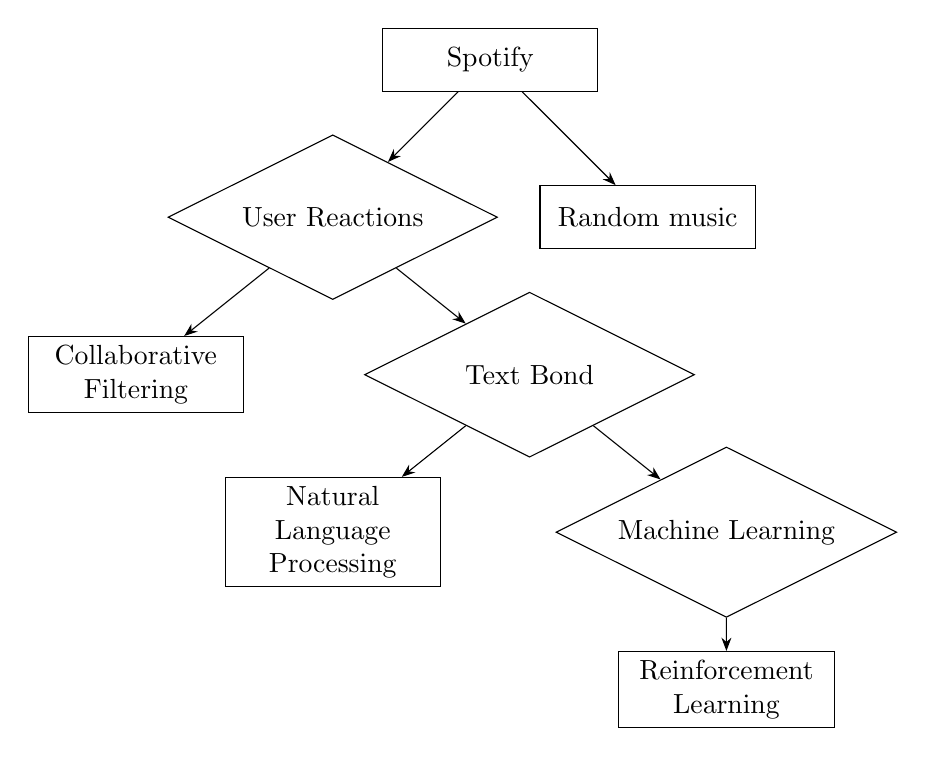
\begin{tikzpicture}[
        level 1/.style={sibling distance=40mm, level distance=20mm},
        level 2/.style={sibling distance=50mm, level distance=20mm},
        every node/.style={draw, rectangle, align=center, minimum height=8mm, minimum width=25mm, text width=25mm},
        decision/.style={diamond, aspect=2, draw, align=center, minimum width=30mm, minimum height=10mm, text width=30mm},
        edge from parent/.style={draw, -{Stealth[]}},
        sibling distance=30mm
        ]
        
        \node {Spotify}
        child {node [decision] {User Reactions}
            child {node {Collaborative Filtering}}
            child {node [decision] {Text Bond}
                child {node {Natural Language Processing}}
                child {node [decision] {Machine Learning} 
                    child {node {Reinforcement Learning}} 
                }
            }
        }
        child {node {Random music}};
    \end{tikzpicture}
\end{center}
\caption{Architecture of spotify's recomendation system}
\label{Schema2}
\end{figure}

\section{An Inside Look: Interview with the Head of Yandex's Recommendation Systems, Danil Burlakov}

    We analyzed an interview with Danil Burlakov, where he explained how the recommendation system of Yandex Music is structured and what technologies are at its core. Our guest has been working on the system for about five years, during which time it went through several leadership changes before Danil himself became the head of the project. A graduate of the Faculty of Mechanics and Mathematics at Moscow State University, Danil now leads the development of recommendation systems for Yandex media services, including Yandex Music\citep{YandexI}.

\subsection{Programming Language Choice}

One of the key points in the interview was the explanation of why Java is used for the recommendation systems at Yandex Music. The recommendation system processes massive data arrays, such as matrices of 10,000 by 1,000, where each cell contains information about user plays, likes, and preferences. Java ensures high performance and efficient handling of multithreaded tasks, which is critical for real-time request processing\citep{YT}.

While Python is popular in machine learning, it is less efficient in handling high loads and large numbers of threads, making it less suitable for tasks that involve processing such large data arrays. For particularly resource-intensive calculations, such as gradient boosting, C++ is used to achieve maximum speed when performing complex operations.

\subsection{Collaborative Filtering and Vector Models}

Collaborative filtering is the primary mechanism behind Yandex Music’s recommendation system. Both users and tracks are represented as vectors. The vector $\vec{A}$ for a user is formed based on their activity, including likes, skips, plays, and genre preferences. The vector $\vec{B}$ for tracks accounts for factors such as genre, popularity, and other characteristics\citep{Yandex}.

For example, if a user frequently listens to electronic and rock music, their vector will be closer to tracks in those genres. When a new track with similar characteristics appears, it will be positioned near the user’s vector, and the system will suggest it in the playlist.

Matrix factorization is used to improve the efficiency of finding relevant tracks. This reduces the dimensionality of the original "users-tracks" matrix, speeding up the process of identifying hidden preferences.

We also developed our own collaborative filtering model in C, which helps optimize the recommendation process and improve system performance (For better understanding we made our model of Colaborative systems, refer to paragraph 5) \footnote{For better understanding, refer to paragraph 5.}.

\subsection{Offline and Online Playlists}

The recommendation system is divided into offline and online playlists. Offline playlists are formed based on long-term user data and are processed in batches, reducing the system’s load. Online playlists are updated instantly, using the most recent data about user plays, likes, and preferences, allowing the system to reflect changes in the user's music taste almost in real-time\citep{lel}\citep{lol}.

\subsection{Data Transfer Protocol and Playlist Updates}

Protocol Buffers (Protobuf) is used to transfer data between services, which is more efficient than JSON. Protobuf reduces data size and speeds up processing, which is crucial when handling millions of users. In Yandex Music, playlists are updated every time the app is opened, allowing the system to consider the user’s latest preferences and adapt to time zone changes. If the user doesn't open the app for a long time, the playlist remains the same, but after a week of inactivity, the data becomes outdated, and the playlist will be updated the next time the user logs in.

Thus, the interview with Danil Burlakov provides a clear understanding of how Yandex Music combines technology and algorithms to create accurate, personalized recommendations.

\section{Comparison}

\begin{table}[h!]
    \centering
    \setlength{\arrayrulewidth}{0.3mm}
    \setlength{\tabcolsep}{8pt}
    \renewcommand{\arraystretch}{1.2}
    
    \newcolumntype{L}[1]{>{\raggedright\arraybackslash}p{#1}}
    \newcommand{\header}[1]{\textbf{\cellcolor[HTML]{D0E5FF}#1}}
    \arrayrulecolor[HTML]{3A75C4}
    
    \resizebox{\textwidth}{!}{
    \begin{tabular}{|L{1.8cm}|L{2.68cm}|L{2.8cm}|L{2.8cm}|L{2.9cm}|}
    \hline
    \header{Criterium} & \header{Apple Music} & \header{Yandex Music} & \header{Spotify} & \header{Deezer} \\ \hline
    \textbf{1 Level}   & Collaborative Filtering & Collaborative Filtering & Collaborative Filtering & Collaborative Filtering \\ \hline
    \textbf{2 Level}   & Natural Language Processing & Matrix Factorization & Natural Language Processing & Natural Language Processing \\ \hline
    \textbf{3 Level}   & Content-Based Filtering & Reinforcement Learning & Reinforcement Learning & Reinforcement Learning \\ \hline
    \textbf{4 Level}   & Reinforcement Learning & Content-Based Filtering & Audio Feature Analysis & Content-Based Filtering \\ \hline
    \end{tabular}
    }
    
    \caption{Comparison\citep{Rick}}
    \label{table1}
\end{table}

\textbf{Similarities}: All four platforms — Apple Music, Yandex Music, Spotify, and Deezer — use collaborative filtering at the first level. This method is based on analyzing user data, such as listening habits, to recommend new tracks by identifying similarities in user preferences. Additionally, for all platforms except Apple Music, reinforcement learning is applied at the third level, allowing them to improve recommendations in real-time based on user interactions with the system (for example, when users skip or replay songs).

\textbf{Differences}: After collaborative filtering, Apple Music applies Natural Language Processing (NLP) to analyze song lyrics or descriptions, then moves to content-based filtering, and concludes the process by using reinforcement learning at the final level.

Yandex Music, after collaborative filtering, uses matrix factorization, which differs from other platforms. This method helps reveal users' hidden preferences. In the following levels, Yandex Music applies reinforcement learning and content-based filtering.

Spotify, after collaborative filtering, also uses Natural Language Processing (NLP) and then applies reinforcement learning. However, at the final stage, Spotify uses audio feature analysis, which includes examining the musical characteristics of tracks, such as tempo, mood, and rhythm.

Deezer, like Spotify, uses Natural Language Processing and reinforcement learning after collaborative filtering, but at the final level, it prefers content-based filtering, similar to Apple Music.

Thus, collaborative filtering and reinforcement learning are key methods used in the early and advanced stages of recommendations for most platforms. However, each platform has unique differences: Yandex Music stands out with its use of matrix factorization, Spotify applies audio feature analysis, while Apple Music and Deezer use content-based filtering at the final level of recommendations.

\section{Colaborative filtering project}

Based on the information I studied, I created a first-level recommendation system using collaborative filtering. To improve accuracy, I surveyed around ten people with different music tastes, who rated tracks on a scale from 0 to 5. Let's break down how the program and cosine similarity work.

\textbf{Program Steps:}
\begin{itemize}
    \item \textbf{Data Collection:} We have user data and their track ratings (from 0 to 5), saved in the file \texttt{UserMarks.txt}. The new user also rates tracks on the same scale.
    
    \item \textbf{Similarity Calculation:} Using cosine similarity, we calculate the similarity coefficient between the new user and each of the users in the database. This coefficient is used to weight the ratings.

    \[
    \cos(\theta) = \frac{A \cdot B}{\|A\| \|B\|}
    \]

    \textbf{Cosine Similarity Formula:} Cosine similarity (the formula above) measures how close the preference vectors of two users are. The closer the value is to 1, the more similar the users’ preferences are.
\begin{lstlisting}
double calculate_coefficient(int* user_ratings, int* song_ratings, int size) {
    double dot_product = 0.0, length_user = 0.0, length_songs = 0.0;
    int valid_count = 0;

    for (int i = 0; i < size; i++) {
        if (user_ratings[i] != -1 && song_ratings[i] != -1) {
            dot_product += (double)user_ratings[i] * song_ratings[i];
            length_user += (double)user_ratings[i] * user_ratings[i];
            length_songs += (double)song_ratings[i] * song_ratings[i];
            valid_count++;
        }
    }

    if (valid_count == 0 || length_songs == 0.0) return 0.0;

    return dot_product / (sqrt(length_user) * sqrt(length_songs));
}
\end{lstlisting}

    In this formula, we find the dot product of the users' ratings, then divide it by the product of the vector lengths (\texttt{length\_user} and \texttt{length\_songs}), normalizing them and producing a coefficient between -1 and 1. This determines how close the preferences are.

    \item \textbf{Calculating the Final Rating:} To recommend a track the new user hasn’t rated, the system uses the following formula:

    \[
    \text{Rating}_{\text{track}} = \frac{\sum_{i=1}^n (\text{UserRating}_i \times \text{SimilarityCoefficient}_i)}{\sum_{i=1}^n \text{SimilarityCoefficient}_i}
    \]

    This formula considers the ratings of all users in the database, weighted by their similarity to the new user.

    \item \textbf{Sorting Recommendations:} We sort tracks by their final ratings, from most to least suitable.
\begin{lstlisting}
void sort_recommendations(double* ratings, char recommendations[MAX_SONGS][255], int size) {
    for (int i = 0; i < size - 1; i++) {
        for (int j = i + 1; j < size; j++) {
            if (ratings[i] < ratings[j]) {
                double temp_rating = ratings[i];
                ratings[i] = ratings[j];
                ratings[j] = temp_rating;
                char temp_song[255];
                strcpy(temp_song, recommendations[i]);
                strcpy(recommendations[i], recommendations[j]);
                strcpy(recommendations[j], temp_song);
            }
        }
    }
}
\end{lstlisting}

    \item \textbf{Outputting Recommendations:} Finally, the program outputs tracks in order from most interesting to least, based on calculated final ratings.
\end{itemize}

This is how collaborative filtering works — by recommending tracks that similar users enjoyed.

\section{Conclusion}
In today’s world of music, where millions of tracks are available at the click of a button, recommendation systems play a key role in shaping our musical experience. Streaming platforms like Yandex Music, Spotify, Apple Music, and Deezer use complex algorithms based on machine learning to tailor music recommendations to individual user tastes.

We explored the main methods used in recommendation systems, including collaborative filtering, natural language processing, and reinforcement learning. Each of these methods offers unique approaches to analyzing listener preferences and providing personalized recommendations. This not only enhances user interaction with the platforms but also fosters the discovery of new music, broadening their musical horizons.

In an interview with Danil Burlakov, we learned about the challenges and future prospects of developing recommendation systems in Yandex Music, as well as how technology and innovation continue to transform the music industry.

Thus, recommendation systems not only simplify the search for music but also actively shape our musical preferences, creating a unique and engaging experience for every listener. In the future, we can expect further refinement of these systems, making them even more accurate and intuitive, while also opening new horizons in the music world.

\newpage
\section{References}

\bibliographystyle{unsrt}  %abbrvnat
\bibliography{MainBIB}

\end{document}











